\documentclass[11pt,a4paper]{article}
\usepackage[T1]{fontenc}
\usepackage[utf8]{inputenc}
\usepackage[sc]{mathpazo}
\linespread{1.04}
\usepackage[scaled=0.86]{helvet}
\usepackage[margin=1in]{geometry}
\usepackage{amsmath,amssymb,amsthm,mathtools}
\usepackage{booktabs}
\usepackage{array}
\usepackage{tabularx}
\usepackage{float}
\usepackage[hidelinks]{hyperref}
\usepackage[nameinlink,noabbrev]{cleveref}
\usepackage{microtype}
\usepackage{enumitem}
\usepackage{siunitx}
\usepackage{xcolor}
\usepackage{caption}
\usepackage{tcolorbox}
\tcbuselibrary{skins,breakable}
\usepackage{thmtools}
\usepackage{tikz}
\usetikzlibrary{arrows.meta,positioning,calc,fit,backgrounds,matrix,decorations.pathmorphing}
\usepackage{pgfplots}
\pgfplotsset{compat=1.18}
\usepackage{longtable}
\usepackage{multirow}
\usepackage{makecell}
\usepackage{bm}
\usepackage{csquotes}
\usepackage{fancyhdr}
\usepackage{titlesec}

% ── Color palette ──
\definecolor{tfptblue}{RGB}{35,60,120}
\definecolor{tfptorange}{RGB}{190,100,20}
\definecolor{tfptgreen}{RGB}{40,110,60}
\definecolor{tfptgray}{RGB}{90,90,95}

\hypersetup{
    colorlinks=true,
    linkcolor=tfptblue!80!black,
    citecolor=tfptblue!70!black,
    urlcolor=tfptblue!60!black,
}

% ── Caption styling ──
\captionsetup{
    font={small,sf},
    labelfont={bf,color=tfptgray},
    labelsep=period,
    margin=1.5em,
    skip=6pt,
}

% ── Section heading styling ──
\titleformat{\section}
    {\Large\bfseries\color{tfptblue}}{\thesection}{0.8em}{}
\titleformat{\subsection}
    {\large\bfseries\color{tfptblue!85!black}}{\thesubsection}{0.7em}{}
\titleformat{\subsubsection}
    {\normalsize\bfseries\color{tfptblue!70!black}}{\thesubsubsection}{0.6em}{}
\titlespacing*{\section}{0pt}{1.8ex plus 0.6ex minus 0.3ex}{0.9ex plus 0.2ex}
\titlespacing*{\subsection}{0pt}{1.4ex plus 0.4ex minus 0.2ex}{0.6ex plus 0.1ex}

% ── Running headers ──
\pagestyle{fancy}
\setlength{\headheight}{22pt}
\fancyhf{}
\fancyhead[L]{\small\itshape\color{tfptgray} TFPT 4.5: Boundary Polarization and Closed-Branch Dynamics}
\fancyhead[R]{\small\color{tfptgray}\thepage}
\renewcommand{\headrulewidth}{0.4pt}
\renewcommand{\headrule}{\hbox to\headwidth{\color{tfptblue!30}\leaders\hrule height \headrulewidth\hfill}}
\fancypagestyle{plain}{\fancyhf{}\fancyfoot[C]{\small\color{tfptgray}\thepage}\renewcommand{\headrulewidth}{0pt}}

% ── tcolorbox global defaults ──
\tcbset{
    enhanced,
    boxrule=0.6pt,
    arc=2.5pt,
    left=6pt, right=6pt, top=5pt, bottom=5pt,
    fonttitle=\bfseries\sffamily\small,
    coltitle=white,
    toptitle=2pt, bottomtitle=2pt,
    shadow={0.8mm}{-0.6mm}{0mm}{black!12},
}

\sisetup{
    detect-all,
    round-mode = none,
    exponent-mode = input,
    exponent-product = \times,
    group-separator = {\,},
    group-minimum-digits = 4
}

\newtheorem{theorem}{Theorem}[section]
\newtheorem{corollary}[theorem]{Corollary}
\newtheorem{lemma}[theorem]{Lemma}
\theoremstyle{definition}
\newtheorem{definition}[theorem]{Definition}
\newtheorem{conjecture}[theorem]{Conjecture}
\newtheorem{proposition}[theorem]{Proposition}
\newtheorem{assumption}[theorem]{Assumption}
\newtheorem{axiom}[theorem]{Axiom}
\newtheorem{principle}[theorem]{Principle}
\newtheorem{construction}[theorem]{Construction}
\newtheorem{claim}[theorem]{Claim}
\newtheorem{appendixstep}[theorem]{Appendix Step}
\theoremstyle{remark}
\newtheorem*{remark}{Remark}

\crefformat{thmt@dummyctr}{Remark}
\Crefformat{thmt@dummyctr}{Remark}
\crefname{thmt@dummyctr}{remark}{remarks}
\Crefname{thmt@dummyctr}{Remark}{Remarks}
\crefname{conjecture}{conjecture}{conjectures}
\Crefname{conjecture}{Conjecture}{Conjectures}
\crefname{definition}{definition}{definitions}
\Crefname{definition}{Definition}{Definitions}

\makeatletter
\def\theHtheorem{\thesection.\thetheorem}
\def\theHcorollary{\theHtheorem}
\def\theHlemma{\theHtheorem}
\def\theHdefinition{\theHtheorem}
\def\theHconjecture{\theHtheorem}
\def\theHproposition{\theHtheorem}
\def\theHassumption{\theHtheorem}
\def\theHprinciple{\theHtheorem}
\def\theHconstruction{\theHtheorem}
\def\theHclaim{\theHtheorem}
\def\theHappendixstep{\theHtheorem}
\makeatother

\DeclareMathOperator{\tr}{Tr}
\DeclareMathOperator{\rank}{rank}
\DeclareMathOperator{\SF}{SF}
\DeclareMathOperator{\Ind}{Ind}
\DeclareMathOperator{\argmin}{arg\,min}

\newcolumntype{Y}{>{\raggedright\arraybackslash}X}

\newcommand{\Seam}{\Sigma}
\newcommand{\inv}{\iota}
\newcommand{\taudbl}{\tau_{\mathrm{dbl}}}
\newcommand{\iC}{\iota_{\mathrm C}}
\newcommand{\epscar}{\varepsilon_{\mathrm{car}}}
\newcommand{\Xbulk}{X_{\mathrm{bulk}}}
\newcommand{\Mpl}{\bar M_{\mathrm{Pl}}}
\newcommand{\Mplunred}{M_{\mathrm{Pl}}}
\newcommand{\cthree}{c_3}
\newcommand{\atheta}{a_\theta}
\newcommand{\phibase}{\varphi_{\mathrm{base}}}
\newcommand{\phiz}{\varphi_0^{\mathrm{ret}}}
\newcommand{\phiseam}{\varphi_{\Sigma}}
\newcommand{\deltatop}{\delta_{\mathrm{top}}}
\newcommand{\omegaCCEW}{\omega_{\mathrm{CC}}^{(2)}}
\newcommand{\bone}{b_1}
\newcommand{\SM}{\mathrm{SM}}
\newcommand{\QCD}{\mathrm{QCD}}
\newcommand{\Oadm}{\Omega_{\mathrm{adm}}}
\newcommand{\Cmin}{\mathcal C_{\min}}
\newcommand{\Ageom}{\mathcal A_{\mathrm{geom}}}
\newcommand{\Atrans}{\mathcal A_{\mathrm{trans}}}
\newcommand{\Arec}{\mathcal A_{\mathrm{rec}}}
\newcommand{\Aobs}{\mathcal A_{\mathrm{obs}}}
\newcommand{\Asing}{\mathcal A_{\mathrm{sing}}}
\newcommand{\Vadm}{\mathcal V_{\mathrm{adm}}}
\newcommand{\Hrel}{\mathcal H_{\mathrm{rel}}}
\newcommand{\Hhad}{\mathcal H_{\mathrm{had}}}
\newcommand{\Hhub}{H_{\mathrm{hub}}}
\newcommand{\Htot}{\mathcal H_{\mathrm{tot}}}
\newcommand{\Gammaeff}{\Gamma_{\mathrm{eff}}}
\newcommand{\lambdaY}{\lambda_Y}
\newcommand{\Pred}{\operatorname{Pred}}
\newcommand{\gcar}{g_{\mathrm{car}}}
\newcommand{\Hint}{\mathcal H_{\mathrm{int}}}
\newcommand{\Kadm}{K_{\mathrm{adm}}}
\newcommand{\Tmin}{\mathfrak T_{\mathrm{min}}}
\newcommand{\Tbound}{\mathfrak T_{\partial}^{\min}}
\newcommand{\Tprim}{\mathfrak T_{\mathrm{prim}}}
\newcommand{\chiseed}{\chi_{\mathrm{seed}}}
\newcommand{\chigeo}{\chi_{\mathrm{geo}}}
\newcommand{\chigeozero}{\chi_{\mathrm{geo},0}}
\newcommand{\APSdom}{\mathrm{APS}_{\mathrm{dom}}}
\newcommand{\APSfam}{\mathrm{APS}_{\mathrm{fam}}}
\newcommand{\vgeo}{v_{\mathrm{geo}}}
\newcommand{\vewref}{v_{\mathrm{EW}}^{\mathrm{ref}}}
\newcommand{\Dstart}{D_{\mathrm{start}}}
\newcommand{\Tcore}{\mathfrak T_{\mathrm{core}}}
\newcommand{\Tbridge}{\mathfrak T_{\mathrm{bridge}}}
\newcommand{\Tker}{\mathfrak T_{\mathrm{ker}}}
\newcommand{\Tcomp}{\mathfrak T_{\mathrm{comp}}}
\newcommand{\Padm}{P_{\mathrm{adm}}}
\newcommand{\Pprim}{P_{\mathrm{prim}}}
\newcommand{\Tpre}{\mathfrak T_{\mathrm{pre}}}
\newcommand{\Tstar}{\mathfrak T_{\star}}
\newcommand{\APSdomprov}{\mathrm{APS}_{\mathrm{dom}}^{\mathrm{prov}}}
\newcommand{\sigmaQCD}{\sigma_{\mathrm{QCD}}}
\newcommand{\Cseam}{\mathcal C_{\Sigma}}
\newcommand{\Ccyc}{\mathfrak C_{\Sigma}}
\newcommand{\Ffals}{\mathsf F_{\mathrm{fals}}}
\newcommand{\Rcmp}{\mathcal R_{\mathrm{cmp}}}
\newcommand{\wspin}{\varpi_{\mathrm{spin}}}
\newcommand{\PhysAdmOne}{\widehat{\mathrm{PhysAdm}}_1}
\newcommand{\ObsAdm}{\mathbf{Obs}_{\mathrm{adm}}}
\newcommand{\GrenTFPT}{\Gamma_{\mathrm{TFPT}}^{\mathrm{ren}}}
\newcommand{\OphysTFPT}{\mathbf O_{\mathrm{phys}}^{\mathrm{TFPT}}}
\newcommand{\OschemeTFPT}{\mathbf O_{\mathrm{scheme}}^{\mathrm{TFPT}}}
\newcommand{\SchGrp}{\mathbf{Sch}}
\newcommand{\Runiv}{\mathfrak R}
\newcommand{\Mop}{\mathfrak M}
\newcommand{\Mphys}{\mathfrak M_{\mathrm{phys}}}
\newcommand{\Mscheme}{\mathfrak M_{\mathrm{scheme}}}
\newcommand{\Rren}{\mathfrak R_{\mathrm{ren}}}
\newcommand{\Bind}{\mathcal B_{\mathrm{ind}}}
\newcommand{\Clrig}{\mathfrak{Cl}}
\newcommand{\Runivrig}{\overline{\Runiv}}
\newcommand{\Seedop}{\mathbf{Seed}^{\mathrm{op}}}
\newcommand{\Cseed}{\mathfrak C_{\mathrm{seed}}}
\newcommand{\triv}{\textup{triv}}
\newcommand{\rankess}{\rank_{\textup{ess}}}
\newcommand{\red}{\textup{red}}


% -- TFPT 4.5 split helpers --
\newcommand{\sourceDraft}{\texttt{../tfpt-42.tex}}
\newcommand{\paperstatus}{Draft split from \sourceDraft; theorem wording still inherits the status discipline of the source manuscript.}

\newenvironment{tfptfrontbox}
{\begin{tcolorbox}[colback=tfptblue!2, colframe=tfptblue!45, breakable,
    title={Scope box: inputs, contribution, non-claims, audit surface}, colbacktitle=tfptblue!65]}
{\end{tcolorbox}}

\newenvironment{tfptwarningbox}
{\begin{tcolorbox}[colback=tfptorange!4, colframe=tfptorange!55, breakable,
    title={Editorial guardrail}, colbacktitle=tfptorange!75]}
{\end{tcolorbox}}

\newenvironment{tfptsourcebox}
{\begin{tcolorbox}[colback=tfptgreen!3, colframe=tfptgreen!50, breakable,
    title={Source extraction map}, colbacktitle=tfptgreen!65]}
{\end{tcolorbox}}

\newcommand{\TFPTxref}[1]{\textup{[TFPT cross-reference: \texttt{\detokenize{#1}}]}}
\newcommand{\TFPTeqref}[1]{\textup{[TFPT equation: \texttt{\detokenize{#1}}]}}

\newenvironment{tfptclaimcontract}
{\begin{tcolorbox}[colback=tfptblue!2, colframe=tfptblue!50, breakable,
    title={Claim contract}, colbacktitle=tfptblue!70]\small}
{\end{tcolorbox}}

\newenvironment{tfptexports}
{\begin{tcolorbox}[colback=tfptgreen!3, colframe=tfptgreen!50, breakable,
    title={Exported objects}, colbacktitle=tfptgreen!65]}
{\end{tcolorbox}}



\title{\color{tfptblue}\textbf{TFPT in One Map}\\[0.4em]
{\Large Boundary Polarization, Carrier Rigidity, and Observable Closure}}
\author{Stefan Hamann \and Alessandro Rizzo}
\date{{\normalsize\color{tfptgray}\sffamily Orientation Note for the TFPT 4.5 paper series -- \today}}

\begin{document}
\maketitle

\begin{abstract}
This note is the thin entry document for the TFPT 4.5 series. It does not attempt to prove the
full theory. Its purpose is to state what TFPT claims, what it does not claim, how the closed branch
is organized, and where each load-bearing argument is isolated in the paper sequence.
\end{abstract}

\begin{tfptfrontbox}
\textbf{Inputs from previous papers.} None. This is the public orientation layer for the series.

\textbf{New theorem contribution.} None. The note contributes only organization, status discipline,
and a dependency map.

\textbf{Not claimed here.} No carrier proof, no exact electromagnetic calculation, no CMB fit, no
mass ledger, no E8 stage atlas, and no nonperturbative QFT proof.

\textbf{Falsification or audit surface.} The note can fail if it misstates the dependency order,
overstates the status of a downstream module, or hides where an assumption first enters.
\end{tfptfrontbox}


\begin{tfptclaimcontract}
\textbf{Claim.} Orientation and dependency map only; no theorem proof.\par
\textbf{Inputs.} None.\par
\textbf{First assumptions.} Status vocabulary and series dependency order.\par
\textbf{Proof status.} Reader contract / orientation.\par
\textbf{Kill condition.} Misstates dependency order or promotes downstream targets to core claims.\par
\end{tfptclaimcontract}

\tableofcontents

\section{What TFPT Claims}

TFPT is organized as a boundary-polarized spectral theory whose primitive input is a one-sided
boundary datum
\[
\Tbound=(\mathcal A_+,\mathcal H_+,D_+,J,\Gamma,B_\Sigma).
\]
The main theorem chain in the source draft is not a collection of unrelated numerological
readouts. It is a staged reconstruction:
\[
\Tbound
\Rightarrow
(\taudbl,\iC,\Pprim,[u_\Sigma],\cthree)
\Rightarrow
d^\star_{\mathrm{disc}}
\Rightarrow
\Padm
\Rightarrow
\mathcal M_{d^\star_{\mathrm{disc}}}
\Rightarrow
\mathcal Z_{\mathrm{cl}}=\{x^\star_{\mathrm{cl}}\}
\Rightarrow
\Tstar .
\]
The split series follows this burden of proof rather than the order in which a reader might find
the numerics exciting.

\section{What TFPT Does Not Claim at This Level}

The orientation note does not certify every downstream comparison row as a theorem. In particular,
the CMB interface, sky-map realization, horizon continuations, transient channels, and E8 scale
grammar remain outside the primitive theorem chain. They are comparison and programmatic layers
unless explicitly promoted by a later proof obligation.

\section{The Three Decoders}

The source manuscript condenses the closed branch through three decoders:
\[
\begin{aligned}
Y&\quad\text{generates structure},\\
[u_\Sigma]=1&\quad\text{generates counting},\\
u:=\phiz&\quad\text{generates bridge observables}.
\end{aligned}
\]
This orientation is the reason the paper series separates the primitive kernel, the carrier
packet, the precision readouts, the QFT closure layer, the metrology layer, and the cosmology
interface.

\section{Status Matrix}

\begin{center}
\begin{tabularx}{\textwidth}{@{}p{0.22\textwidth}p{0.22\textwidth}Y@{}}
\toprule
\textbf{Layer} & \textbf{Status language} & \textbf{Where handled} \\
\midrule
Boundary primitive kernel & Theorem-level target & Paper 1 \\
Carrier rigidity and SM packet & Theorem-level target with representation audit & Paper 2 \\
Electromagnetic and flavor readouts & Closed-branch prediction layer with no-knobs audit & Paper 3 \\
Admissibility and QFT closure & Conditional nonperturbative closure under stated hypotheses & Paper 4 \\
Boundary-normalized metrology & Dimensionless observable functor from $\lambda_\Sigma$ & Paper 5 \\
Cosmology and CMB & Downstream interface; Stage 1 spectra, Stage 2 sky realization target & Paper 6 \\
Extended comparison maps & Appendix and companion material & Technical Companion \\
\bottomrule
\end{tabularx}
\end{center}

\section{Series Map}

\begin{enumerate}[leftmargin=1.5em]
    \item \textbf{Boundary Polarization and the Primitive Kernel of TFPT.}
    Establishes $\Tbound\Rightarrow(\taudbl,\iC,\Pprim,[u_\Sigma],\cthree)$ and keeps all
    Standard-Model claims out.
    \item \textbf{Carrier Rigidity, Hypercharge, and the Standard Model Packet from Boundary
    Polarization.}
    Establishes the rigid $3+2$ carrier, hypercharge, $S^+=\Lambda^{\mathrm{even}}E$,
    $G_{\mathrm{phys}}$, $N_{\mathrm{fam}}=3$, $\Omega_{\mathrm{adm}}=48$, $N_\Phi=1$, and
    $\bone=41/10$.
    \item \textbf{Electromagnetic Fixed Point and Flavor Transport on the Rigid TFPT Branch.}
    Isolates $\alpha$, $\delta_{\mathrm{ph}}$, $\lambda_C$, $\beta_{\mathrm{rad}}$, $\Omega_b$,
    $\theta_{13}$, CKM, and PMNS.
    \item \textbf{Admissibility, Strong CP, and Nonperturbative QFT Closure on the TFPT Branch.}
    Separates selector from dynamics and states the positivity, OS, local-net, scattering, and
    exact-flow obligations.
    \item \textbf{Geometric Hodge Closure and Dimensionless Metrology from the TFPT Boundary
    Branch.}
    Treats $\lambda_\Sigma$, Planck normalization, electroweak matching, and boundary-normalized
    observables.
    \item \textbf{Cosmology Interfaces of the TFPT Closed Branch.}
    Treats seam transfer, determinant-line phase, axion sector, reheating, leptogenesis, CMB
    spectra, and sky-realization targets.
\end{enumerate}

\section{Publication Order}

The recommended public order is Paper 0, Paper 2, Paper 1, Paper 3, Paper 4, Paper 5, and finally
Paper 6. The mathematical dependency order remains Paper 1 before Paper 2; the publication order
uses Paper 2 as the clearest visible hook while Paper 0 explains the dependency discipline.

\section{Source Boundary}

\begin{tfptsourcebox}
Primary source: \sourceDraft.

The orientation note draws especially from the abstract, the closed-architecture box, Sections 1
and 2, the canonical rigid-object discussion, the structural falsification map, and the conclusion.
It intentionally does not import the extended empirical ledgers, E8 stage atlas, CMB figures, or
mass tables.
\end{tfptsourcebox}

\clearpage
\section{Main Technical Development}

This section contains the main technical development assigned to this paper by the TFPT 4.5 clean split. Cross-paper background is referenced through dependency and scope boxes; extended backend material is kept in the Technical Companion.

% Auto-extracted from ../tfpt-42.tex for the TFPT 4.5 clean split.
% Source body assigned by the TFPT 4.5 clean split.

% ---- Original abstract, closed architecture, reading guide, and big picture: source lines 235-848 ----
\begin{abstract}
From the one-sided boundary datum
\[
\Tbound=(\mathcal A_+,\mathcal H_+,D_+,J,\Gamma,B_\Sigma),
\]
the manuscript derives the Calder\'on polarization $P_C$, the boundary involution
$\iC:=2P_C-1$, the exact-double deck involution $\taudbl$, and the doubled closed datum
\[
\Tmin^{\mathrm{cl}}=(\mathcal A,\mathcal H,D,J,\Gamma,\taudbl,\iC).
\]
The hard core is now read through three decoders. First, the carrier decoder $Y$ satisfies
\[
6Y^2-Y-\mathbf 1=0,
\qquad
\tr_EY=0,
\]
and in the primitive realization forces the rigid $3+2$ carrier split
$E=E_3\oplus E_2$, the primitive two-point generator $X=6Y$, the one-family packet
$S^+=\Lambda^{\mathrm{even}}E$, and the physical gauge quotient
\[
G_{\mathrm{phys}}
=
\frac{SU(3)\times SU(2)\times U(1)_Y}{\mathbb Z_6}.
\]
Second, the global winding decoder $[u_\Sigma]=1$ fixes the rigid family surface
$X_f^\circ\cong \mathbb P^1\setminus\mu_4$, yields the minimal family repair
\[
16\gamma=\frac{40}{3}
\qquad\Longrightarrow\qquad
N_{\mathrm{fam}}=3,
\qquad
\Omega_{\mathrm{adm}}=48,
\]
and, on the transport branch, fixes the intrinsic pole as the lower critical point of the cusp cubic
\[
P(z)=(z-1)\left(z-\frac{64}{729}\right)\left(z-\frac{1}{729}\right),
\qquad
P'(z)=0.
\]
Third, the retained seed decoder
\[
u:=\varphi_0^{\mathrm{ret}}
\]
projects simultaneously to $(\lambda_C,\beta_{\mathrm{rad}},\Omega_b,\theta_{13})$, while the
closed transport-plus-Higgs budget
\[
\sum_{f,j}L_{f,j}^{\mathrm{diag}}+N_\Phi=41
\]
closes the exact electromagnetic fixed point $\alpha$.

The theorem flow is therefore no longer presented as a strictly linear carrier-then-family arrow
chain. After the boundary datum has fixed the doubled primitive reconstruction, the primitive seam
generator, and the primitive Hodge selector, the manuscript solves one joint discrete admissibility
problem and only afterwards the continuous Euler--Lagrange problem:
\[
\Tbound
\;\Rightarrow\;
(\taudbl,\iC,\Pprim,[u_\Sigma],\cthree)
\;\Rightarrow\;
d^\star_{\mathrm{disc}}
\;\Rightarrow\;
\Padm
\;\Rightarrow\;
\mathcal M_{d^\star_{\mathrm{disc}}}
\;\Rightarrow\;
\mathcal Z_{\mathrm{cl}}=\{x^\star_{\mathrm{cl}}\}
\;\Rightarrow\;
\Tstar.
\]
Here the unique discrete datum is
\[
d^\star_{\mathrm{disc}}
:=
\bigl(
E_3\oplus E_2,\,
Y,\,
S^+,\,
X_f^\circ,\,
[\nabla_F^\star],\,
c_1(L_2),\,
c_1(L_3),\,
N_{\mathrm{fam}}=3,\,
\theta_{\mathrm{eff}}=0
\bigr),
\]
so carrier, family, determinant data, and strong CP are fixed jointly from one boundary primitive
kernel rather than in a one-way family-after-carrier rhetoric. Here $\Padm:=\Pi_{\ker
\Delta_{\mathrm{adm}}}$ selects the physical admissible sector, while the actual dynamics is
carried by the relative generating functional $Z_{\mathrm{rel}}$, the admissible Schwinger
distributions, the Osterwalder--Schrader reconstruction, the local Minkowski net on the admissible
Hilbert space, the exact admissible flow $\Gamma_k$, and its infrared limit
$\Gamma_{\mathrm{TFPT}}^{\mathrm{ren}}$.

The same seam transfer, determinant-line phase, and scalaron sector then fix the closed-branch
cosmology interface data from which infrared continuation, reheating, and leptogenesis readouts are
computed. Two further structural maps are attached strictly outside the theorem chain: the
structural falsification map $\Ffals(\Tstar)$ in the main text and the appendix-level comparison
map $\Rcmp(\Tstar)$. Above the rigid core, the manuscript records an internal reduction on the
weakened ambient class $\PhysAdmOne$, an internal renormalized low-energy layer $\GrenTFPT$, and a
reality-first observable stratification
\[
\Tstar\;\xrightarrow{\Rren}\;\GrenTFPT\;\xrightarrow{\Mphys}\;\OphysTFPT
\;\xrightarrow{\Mscheme}\;\OschemeTFPT/\SchGrp.
\]
This output layer is read in boundary-normalized form: with
\[
\lambda_\Sigma:=\lambda_1^+(|B_\Sigma|),
\qquad
\frac{O}{\lambda_\Sigma^{d_O}}=\mathcal F_O(\Tstar),
\]
so dimensionless gravitational, electroweak, pole-mass, flavor-ratio, and infrared readouts are
internal branch outputs rather than external metrological inputs.
The final theorem-level claim is the canonical rigid object of the boundary-polarized branch, the
admissible QFT closure on the retained sector, and the renormalized physical observable layer, with
cosmology carried at the level of closed-branch interface data and appendix comparison
continuations. In the condensed decoder reading,
\[
\begin{aligned}
Y&\ \text{generates structure},\\
[u_\Sigma]=1&\ \text{generates counting},\\
u&\ \text{generates bridge observables}.
\end{aligned}
\]
\end{abstract}

\begin{tcolorbox}[colback=tfptblue!2, colframe=tfptblue!40, breakable,
    title={Closed architecture of the paper}, colbacktitle=tfptblue!60]
\[
\PhysAdmOne
\xrightarrow{\Runivrig}
\mathbf{TFPT}^{\mathrm{rig}}
\simeq
\{\Tstar\}
\xrightarrow{\Rren}
\GrenTFPT
\xrightarrow{\Mphys}
\OphysTFPT
\xrightarrow{\Mscheme}
\OschemeTFPT/\SchGrp.
\]
Main theorem stack:
\[
\begin{aligned}
\mathfrak S_{\min}
&\;\Rightarrow\;
\mathcal B_{\min}
\;\Rightarrow\;
\Tbound
\;\Rightarrow\;
(\taudbl,\iC,\Pprim,[u_\Sigma],\cthree)
\;\Rightarrow\;
d^\star_{\mathrm{disc}}
\\
&\;\Rightarrow\;
\Padm
\;\Rightarrow\;
\mathcal M_{d^\star_{\mathrm{disc}}}
\;\Rightarrow\;
\mathcal Z_{\mathrm{cl}}=\{x^\star_{\mathrm{cl}}\}
\;\Rightarrow\;
\Tstar.
\end{aligned}
\]
Compressed decoder reading:
\[
\begin{aligned}
Y&\ \text{generates structure},\\
[u_\Sigma]=1&\ \text{generates counting},\\
u:=\phiz&\ \text{generates bridge observables}.
\end{aligned}
\]
\[
\begin{aligned}
6Y^2-Y-\mathbf 1=0,\ \tr Y=0
&\Rightarrow
E_3\oplus E_2,\ S^+,\ \gamma=\frac56,\\
16\gamma=\frac{40}{3}
&\Rightarrow
N_{\mathrm{fam}}=3
\Rightarrow
\Omega_{\mathrm{adm}}=48.
\end{aligned}
\]
\[
P'(z)=0
\Rightarrow
\delta_{\mathrm{ph}},
\qquad
\sum_{f,j}L_{f,j}^{\mathrm{diag}}+N_\Phi=41
\Rightarrow
\alpha.
\]
The input-side reduction to $\Tstar$ and the internal passage from $\Tstar$ to $\GrenTFPT$ and
$\OphysTFPT$ are theorem-level. Only the final projection to $\OschemeTFPT/\SchGrp$ is an
appendix-facing interface. From $\Tstar$ the structural falsification map $\Ffals(\Tstar)$ stays in
the main text, while the comparison map $\Rcmp(\Tstar)$ together with thresholds, schemes, and
empirical rows is collected only in the appendix-level empirical readout.
\end{tcolorbox}

\tableofcontents

\section{Reading guide and claim map}

The paper is organized in three reading layers:
\begin{itemize}[leftmargin=1.5em, topsep=3pt, itemsep=2pt]
    \item \textbf{Big picture:} one section explains what TFPT claims in plain language before the detailed datum and conventions begin.
    \item \textbf{Detail:} the main body then runs from boundary polarization and hard carrier rigidity through kernel numerics, the two closure-architecture sections, the closure theorem stack, the canonical rigid object, the seam-transfer cosmology block, and the internal-reduction / readout-organization section, while the appendix-level empirical readout may be read afterwards.
    \item \textbf{Proof-complete core:} the load-bearing completion theorems are proved in full in the manuscript.
    The appendices keep manuscript-level analytic proofs, auxiliary elaborations, optional
    continuations, and interface tables, but they are not needed for the logical closure of the
    primitive kernel, the continuous master functional, or the canonical rigid object.
\end{itemize}
The role language is also fixed once and for all:
\begin{itemize}[leftmargin=1.5em, topsep=3pt, itemsep=2pt]
    \item \textbf{Boundary datum} means the one-sided theorem package $\Tbound$ induced by the minimal operational seed and used downstream to reconstruct the Calder\'on polarization, doubled closed datum, and admissibility projector. The later minimal-packaging theorem shows that no extra primitive discrete datum is needed beyond it.
    \item \textbf{Theorem} means a statement proved directly from the operational-seed / boundary-datum chain and earlier theorem-level outputs.
    \item \textbf{Derived consequence} means a downstream structural output obtained by composing already proved theorems without introducing a new datum.
\end{itemize}
Below theorem level the manuscript uses only five auxiliary tags:
\begin{itemize}[leftmargin=1.5em, topsep=3pt, itemsep=2pt]
    \item \textbf{Exact identity} means an algebraic equality on an already fixed branch or kernel package.
    \item \textbf{Derived consequence} means a nonprimitive output obtained by composing earlier theorem-level statements.
    \item \textbf{Appendix continuation} means a downstream numerical or conceptual extension that requires one extra assumption beyond the main theorem surface.
    \item \textbf{Programmatic closure target} means a mathematically precise downstream target whose statement is fixed clearly enough to define a falsifiable obligation, but whose proof is not claimed in the present version.
    \item \textbf{Interpretive reading} means a heuristic or explanatory picture not used as theorem input.
\end{itemize}
Comparison conventions are isolated in the appendix-level empirical interface and are not used as
main-text theorem labels. To keep theorem language, benchmark semantics, and appendix bookkeeping
lexically stable, all prose, captions, and role labels are kept in English throughout.

\subsection{Version 4.5 completion surface}

The manuscript now contains a fully rigid algebraic core together with analytic closure blocks
whose exact status is recorded theorem by theorem in the proof-obligation ledger. The remaining
explicit standard-theorem interface is
\[
O_{7\mathrm{d,0}},
\]
while the other former $B/C$ interfaces have now been pulled into the manuscript proof surface. The
eight items below are therefore not a promise of later completion; they are the status-coded 4.5
surface of the present manuscript.

\begin{tcolorbox}[colback=tfptblue!2, colframe=tfptblue!40, breakable,
    title={Version 4.5 completion surface}, colbacktitle=tfptblue!60]
\begin{enumerate}[leftmargin=1.5em, topsep=3pt, itemsep=4pt]
    \item \textbf{[A] Operational seed generation of the one-sided boundary datum.} Introduce the thinner operational seed class $\Seedop$ and prove that it functorially induces the one-sided admissible boundary datum. Proof architecture: reflection positivity and the collar generator reconstruct the one-sided OS Hilbert space and adapted boundary operator, while the seam class induces the spectral-flow datum.
    \item \textbf{[A] Minimal packaging inside the induced admissible boundary class.} Organize the induced one-sided boundary class by lexicographic minimality without hiding a second primitive discrete layer. Proof architecture: lexicographic minimality of seam winding, finite primitive carrier rank, corner count, determinant charge, and boundary kernel dimension; collar product form then yields the one-sided boundary operator and reflection-positive doubling.
    \item \textbf{[A] $D_4$ Riemann--Hilbert rigidity theorem.} Close the family-holonomy debt by fixing the four puncture loops, the local $\{1,\omega,\omega^2\}$ conjugacy classes, the trivial determinant line, and the full $D_4$ puncture symmetry. Proof architecture: monodromy is forced up to global $SU(3)_F$ conjugation, then Riemann--Hilbert yields the unique flat Hermitian family-connection class.
    \item \textbf{[A] Compact determinant and Higgs index theorem.} Promote the determinant-line / Higgs block from a near-complete closure to a compact Dolbeault index theorem on the seam-normal sphere. Proof architecture: $(c_1(L_2),c_1(L_3))=(1,0)$ gives $L_2\cong\mathcal O(1)$ and $L_3\cong\mathcal O$, so Birkhoff--Grothendieck and Riemann--Roch force exactly one weak doublet and no light color triplet.
    \item \textbf{[A] Canonical transport-kernel theorem.} Recast the transport block at theorem level in operator language rather than in path rhetoric. Proof architecture: the structural kernel $K_f^{\mathrm{str}}$ together with the rigid family holonomy produces the Yukawa matrices in the canonical family basis; the primitive indecomposable Yukawa generator then forces the rigid $3+2$ carrier split.
    \item \textbf{[A] Stratified master-functional theorem.} Replace the last appearance of separate closure stories by one stratified functional on admissible spectral bordisms. Proof architecture: a lexicographic barrier fixes the minimal discrete stratum, while the relative partition function, zeta determinant, and eta term generate the continuous Euler--Lagrange equations on the retained branch.
    \item \textbf{[A] Spectral UV completion and renormalized 1PI readout theorem.} Close the continuum side at the spectral rather than purely local Einstein level. Proof architecture: a positive-kernel Birkhoff contraction fixes the unique admissible UV profile, Stieltjes form factors give the ghost-free two-point gravitational kernel, the projective-limit measure supplies the constructive UV object, and the renormalized observable hierarchy is read as the exact 1PI / Legendre layer of the same admissible measure.
    \item \textbf{[A] Absolute spectral Planck closure and stationary vacuum theorem.} Fix the boundary spectral unit $\lambda_\Sigma$, the unique stationary root $\rho_\star$ of the boundary-normalized gravitational functional, and the resulting reduced-Planck / Newton / Schwarzschild--de Sitter readouts directly on the main theorem surface.
    \item \textbf{[A] FRW reduction and cosmology interface theorem.} Turn seam transfer, determinant-line dynamics, and the scalaron sector into one reduced low-curvature action together with explicit cosmology interface data. Proof architecture: homogeneous/isotropic reduction in $(a,\phi,\theta_\Sigma,N_i)$ yields $\Lambda_{\mathrm{IR}}$, the axion displacement data, and the reheating / leptogenesis input block on the same admissible branch, while the final nonequilibrium readouts remain comparison-layer outputs.
\end{enumerate}
\end{tcolorbox}

\begin{remark}[Remaining interface for the 4.5 map]
The target blocks above are now accompanied by only one explicit standard-theorem interface that
should remain visible rather than absorbed into rhetoric: the infrared-dressed massless scattering
interface on the low-curvature branch ($O_{7\mathrm{d,0}}$). The OS/CAR reconstruction, massive
Haag--Ruelle / LSZ closure, and the FRW cosmology interface are now carried by manuscript-level
appendix proofs.
\end{remark}

\begin{remark}[Status of the 4.5 completion surface]
The nine theorem blocks above are integrated into the manuscript, but their exact status is still
recorded line by line in the proof-obligation ledger. The point is therefore not rhetorical
completion language but synchronized proof metadata.
\end{remark}

\begin{tcolorbox}[colback=tfptblue!2, colframe=tfptblue!40, breakable,
    title={Extended downstream closure surface}, colbacktitle=tfptblue!60]
\begin{enumerate}[leftmargin=1.5em, topsep=3pt, itemsep=4pt]
    \item \textbf{[P] Horizon modular thermality and compact-object thermodynamics.} Upgrade the split-inclusion horizon package to stationary modular flow, Hawking temperature, Wald entropy, and Kerr / scalaron correction bounds on the vacuum branch.
    \item \textbf{[P] Primordial perturbation closure from the seam state.} Fix the reheating $e$-fold number, seam-state Bogoliubov data, and Mukhanov--Sasaki / tensor initial conditions on the closed branch.
    \item \textbf{[P] CMB transfer, baryogenesis, and late-time matter readout.} Carry the seam-fixed primordial spectrum through the transfer hierarchy, the flavored Boltzmann system, and the late-time $H_0$ / $P_m(k,z)$ readouts.
    \item \textbf{[P] Late-time dark-sector structure and relative vacuum-energy control.} Record the axion Schr\"odinger--Poisson branch and the finite relative admissible vacuum-energy formula as the late-time dark-sector closure target.
    \item \textbf{[P] Pole-mass completion and Higgs readout.} Read quark / lepton pole masses and the Higgs pole from the admissible RG branch rather than from source rows or raw UV data.
    \item \textbf{[P] Admissible code subspace and pointer dynamics.} Promote the appendix record / Born machinery to a global code-subspace reading of entanglement, pointer stability, and record growth on $\mathcal H_{\mathrm{adm}}$.
    \item \textbf{[P] Topological transient channels.} Keep phase-slip burst phenomenology as a precise falsifiable transient target without promoting it to theorem status.
\end{enumerate}
\end{tcolorbox}

\begin{tcolorbox}[colback=tfptblue!2, colframe=tfptblue!40, breakable,
    title={Closed theorem surface}, colbacktitle=tfptblue!60]
\begin{itemize}[leftmargin=1.5em, topsep=3pt, itemsep=3pt]
    \item \textbf{Initial layer:} the minimal operational seed $\mathfrak S_{\min}$ induces the minimal admissible bordism $\mathcal B_{\min}$ and hence the one-sided boundary datum $\Tbound$.
    \item \textbf{Boundary datum:} $\Tbound$ with one-sided center, self-adjoint boundary operator, seam collar, and canonical doubling data.
    \item \textbf{Theorem layer I:} doubling / deck involution / boundary polarization $\bigl(\taudbl,\iC\bigr)$, the doubled primitive reconstruction $\Tprim$, and the primitive Hodge projector $\Pprim$ from the Calder\'on projector, APS realization, and $D_{\mathrm{rel}}$.
    \item \textbf{Theorem layer II:} the primitive winding class $[u_\Sigma]=1$ and the rigid $D_4$
    family geometry fix $X_f^\circ\cong\mathbb P^1\setminus\mu_4$ and $N_{\mathrm{fam}}=3$; the
    trace-balanced carrier decoder $6Y^2-Y-\mathbf 1=0$, $\tr Y=0$ is realized minimally as the
    rigid $3+2$ carrier kernel $E_3\oplus E_2$, the primitive hypercharge generator $Y$, the
    one-family packet $S^+$, and $\gamma=5/6$; together with the compact Higgs index this fixes
    $\Omega_{\mathrm{adm}}=48$, the determinant class $(c_1(L_2),c_1(L_3))=(1,0)$, and
    $\theta_{\mathrm{eff}}=0$.
    \item \textbf{Theorem layer III:} after the discrete datum has been fixed, the full selector
    $\Padm$ and the projected modular free energy determine the electromagnetic, geometric,
    transport, and vacuum sectors as one continuous Euler--Lagrange problem; on the retained branch
    this is read as $\lambda_\Sigma=\lambda_1^+(|B_\Sigma|)$,
    $\partial_\rho\widehat V_{\mathrm{Pl}}^{\mathrm{ren}}(\rho_\star)=0\Rightarrow(\Mpl/\lambda_\Sigma,\ G_N\lambda_\Sigma^2)$,
    $P'(z)=0\Rightarrow\delta_{\mathrm{ph}}$,
    $u:=\phiz\Rightarrow(\lambda_C,\beta_{\mathrm{rad}},\Omega_b,\theta_{13})$, and
    $\sum_{f,j}L_{f,j}^{\mathrm{diag}}+N_\Phi=41\Rightarrow\alpha$.
    \item \textbf{Theorem layer IV:} the intrinsic branch is the singleton fiber product of the discrete
    sector and the four continuous sector solution sets; from this follow internal analytic closure,
    essential injectivity on the rigid image, and the canonical rigid object $\Tstar$.
    \item \textbf{Input/output layer:} internal reduction $\Runiv$ from $\PhysAdmOne$ to the rigid TFPT class is proved on the input side; the renormalized observable chain $\Tstar\to\GrenTFPT\to\OphysTFPT$ is theorem-level on the output side; only the final scheme projection to $\OschemeTFPT/\SchGrp$ remains appendix-facing.
    \item \textbf{Side maps:} a structural falsification map $\Ffals(\Tstar)$ in the main text, and an appendix-only comparison map $\Rcmp(\Tstar)$ for thresholds, schemes, and empirical rows after the physical observable layer has already been fixed.
\end{itemize}
\end{tcolorbox}

\begin{figure}[t]
\centering
\begin{tikzpicture}[
    scale=0.50,
    transform shape,
    >=Latex,
    node distance=1.45cm and 1.25cm,
    datum/.style={draw=gray!70!black, thick, rounded corners, fill=gray!10, align=center, minimum width=2.55cm, minimum height=1cm},
    main/.style={draw=blue!60!black, thick, rounded corners, fill=blue!6, align=center, minimum width=2.7cm, minimum height=1cm},
    star/.style={draw=blue!70!black, very thick, rounded corners, fill=blue!12, align=center, minimum width=2.7cm, minimum height=1cm},
    falsside/.style={draw=orange!70!black, thick, rounded corners, fill=orange!8, align=center, minimum width=3.1cm, minimum height=0.95cm},
    appendix/.style={draw=green!50!black, dashed, line width=0.8pt, rounded corners, fill=green!4, align=center, minimum width=3.1cm, minimum height=0.95cm}
]
\node[datum] (core) {boundary datum\\$\Tbound$};
\node[main, right=of core] (prim) {boundary primitive kernel\\$\taudbl,\ \iC,\ \Pprim,\ [u_\Sigma],\ \cthree$};
\node[main, right=of prim] (disc) {joint decoder datum\\$Y,\ [u_\Sigma],\ u$};
\node[main, right=of disc] (closure) {selector + master functional\\$\Padm,\ \mathcal M_{d^\star_{\mathrm{disc}}}$};
\node[main, right=of closure] (branch) {singleton branch\\$\mathcal Z_{\mathrm{cl}}=\{x^\star_{\mathrm{cl}}\}$};
\node[star, right=of branch] (out) {canonical rigid object\\$\Tstar$};
\node[falsside, below=of branch] (fals) {structural falsification map\\$\Ffals(\Tstar)$ (main text)};
\node[appendix, below=of out] (cmp) {appendix comparison map\\$\Rcmp(\Tstar)$, schemes, ledgers};
\draw[->, thick] (core) -- (prim);
\draw[->, thick] (prim) -- (disc);
\draw[->, thick] (disc) -- (closure);
\draw[->, thick] (closure) -- (branch);
\draw[->, thick] (branch) -- (out);
\draw[->, thick, orange!70!black] (out.south) .. controls +(0,-0.6) and +(1.1,0.3) .. (fals.east);
\draw[->, dashed, line width=0.8pt, green!50!black] (out.south) .. controls +(0,-1.0) and +(0,0.5) .. (cmp.north);
\end{tikzpicture}
\caption{Closed dependency map with decoder core.}
\label{fig:dependency-map}
\end{figure}

\begin{table}[t]
\centering
\scriptsize
\begin{tabularx}{\linewidth}{@{}>{\raggedright\arraybackslash}p{0.24\linewidth}>{\raggedright\arraybackslash}p{0.13\linewidth}YY@{}}
\toprule
Layer or statement & Role & Proof source or remaining note & Main structural test or falsifier \\
\midrule
Operational seed generation, minimal packaging, and boundary datum $\Tbound$ & Boundary datum & operational-seed theorem, minimal-packaging theorem, and Calder\'on polarization theorem & failure would collapse the operator-level starting point \\
Doubling data $\taudbl$, boundary polarization $\iC$, doubled scaffold, and seam & Theorem & doubling / deck-involution / Calder\'on polarization theorem in the main text & structural consistency of every later theorem \\
Canonical admissibility projector $\Padm$ & Theorem & canonical admissibility complex and Hodge projector lemma & unified electroweak / QCD / CP / gravity selection must survive one common projector \\
Carrier decoder $Y$, bosonic rank-two closure, branch Yukawa rigidity, and one-family packet $S^+$ & Theorem & algebraic normal-form lemma, primitive trace-balanced carrier lemma, compact Higgs index corollary, branch Yukawa rigidity theorem, exterior-packet decomposition, and derived $48=4\cdot12$ identity & group/matter mismatch would be global \\
Winding decoder $[u_\Sigma]=1$, $\mathcal H_F\cong F\cong\mathbb C^3$, and $\Oadm=48$ & Theorem & four-corner / four-puncture theorem, harmonic family-mode theorem, family-integrality-repair corollary, and occupancy corollary & flavor multiplicity must be fixed without extra family input \\
Determinant classes and unique Higgs doublet & Theorem & minimal clutching theorem and compact bosonic index on the seam normal sphere & any unavoidable extra light triplet would falsify the theorem \\
Electromagnetic fixed point, retained-seed decoder, exact charged-lepton ratios, and closed $41$ chain & Theorem & stationary $U(1)$ effective action, retained-seed decoder proposition, mass-compression theorem, and family/Higgs specialization & failure would break the fixed-point equation or the exact seed compression \\
Geometric Hodge gravity sector, boundary spectral unit, absolute spectral Planck closure, and low-curvature spectral branch & Theorem & spectral Einstein functional, boundary spectral-unit rigidity, absolute spectral Planck closure, Schwarzschild--de Sitter corollary, sectorial Hamilton decomposition, constructive geometric measure theorem, and spectral UV completion theorem & inability to obtain one coupled gravity/Higgs closure with one boundary-normalized stationary root would break the branch \\
$D_4$ family minimization, rigid family holonomy, cubic transport decoder, and residue--winding transport closure & Theorem & variational family theorem, monodromy-rigidity theorem, algebraic transport-pole theorem, regularized transport-pole stability lemma, exact $C_6$ resolvent, hard holonomy theorem, and winding sum rule & hierarchy grammar and winding lock must agree on one packet set \\
Determinant-line phase and strong-CP closure & Theorem & positive polar decomposition, determinant-line phase theorem, and admissible vacuum positivity & a stable nonzero effective strong-CP angle would falsify the theorem \\
FRW reduction, seam transfer, and cosmology interface data & Theorem & seam-transfer theorem, boundary-winding theorem, FRW/interface theorem, determinant-line axion interface theorem, and leptogenesis-interface theorem & positive trace-class seam transfer and scalaron closure must persist \\
Canonical rigid object and uniqueness & Theorem & internal analytic closure, essential injectivity on the rigid image, and canonical-object corollary & existence of a second nonisomorphic rigid realization would falsify the theorem \\
Internal reduction on the weakened ambient class $\PhysAdmOne$ & Theorem & weakened ambient admissibility category, internal carrier / family / transport reductions, canonical rigid closure, and uniqueness theorem & existence of a physically admissible candidate in $\PhysAdmOne$ not closing canonically to $\Tstar$ would falsify the theorem \\
Renormalized observable hierarchy and scheme projection discipline & Theorem & admissible 1PI package, renormalized observable theorem, physical observable factorization, minimal observable basis, and appendix scheme conventions & existence of an admissible observable not factoring through $\GrenTFPT\to\OphysTFPT$ or a hidden fit parameter outside $\SchGrp$ would falsify the theorem \\
\bottomrule
\end{tabularx}
\caption{Closed theorem surface for the present version. Internal reduction and the passage to the renormalized and physical observable layers are theorem-level; only the final scheme projection remains an appendix-facing interface. Comparison conventions, threshold rows, and empirical ledgers stay isolated in the appendix-level readout.}
\label{tab:status-matrix}
\end{table}

The family closure used throughout the main text is now read as topologically fixed, variationally
stabilized, and canonically compatible with the doubled admissible branch; no separate family datum
remains outside the theorem surface. Likewise the finite chiral packet condition
$\dim\Lambda^{\mathrm{even}}E=16$ is no longer left as ambient residue but is reconstructed
internally by the bosonic-rank and branch-Yukawa carrier closure.

\section{Big picture: what TFPT actually claims}

TFPT is presented here as a boundary-polarized closed theory of admissible vacua on the oriented
double cover. The formal theorem stack now starts from a thinner operational seed which functorially
induces the one-sided boundary datum, and the manuscript also shows that within the induced
boundary class no extra primitive discrete datum is needed. On the
one-sided branch, the self-adjoint boundary operator $B_\Sigma$ determines the Calder\'on projector,
the Calder\'on projector determines the seam polarization
$\iC$, and the canonical doubling then reconstructs the doubled scaffold $\Tprim$ together with
the primitive Hodge projector $\Pprim$. From this boundary kernel the manuscript next solves one
joint discrete admissibility problem, now best read through three decoders. The trace-balanced
carrier decoder
\[
6Y^2-Y-\mathbf 1=0,
\qquad
\tr Y=0
\]
fixes the rigid $E_3\oplus E_2$ split, hypercharge, and the one-family packet $S^+$. The global
winding decoder $[u_\Sigma]=1$ fixes the rigid family surface $X_f^\circ\cong\mathbb P^1\setminus
\mu_4$, the minimal family count $N_{\mathrm{fam}}=3$, and the admissible occupancy
$\Omega_{\mathrm{adm}}=48$. On the retained branch the seed decoder
\[
u:=\phiz
\]
simultaneously bridges $(\lambda_C,\beta_{\mathrm{rad}},\Omega_b,\theta_{13})$, while
$P'(z)=0$ fixes the intrinsic transport pole and the closed budget
$\sum_{f,j}L_{f,j}^{\mathrm{diag}}+N_\Phi=41$ closes the electromagnetic fixed point $\alpha$.
Only after that discrete theorem is the selector promoted to its full form
$\Padm=\Pprim P_{\mathrm{sing}}P_{\Theta}$, and the projected modular free energy drives the
continuous electromagnetic, geometric, transport, and vacuum closure: the geometric Hodge sector
yields the gravity/scalaron branch, and the exact transport grammar emits Yukawas, hadronic
admissibility, and strong-CP closure on the same admissible branch. The resulting theorem stack
does not merely emit a closed output package; it characterizes a canonical rigid object $\Tstar$ in
the rigid TFPT theorem class. The structural falsification map $\Ffals(\Tstar)$ stays in the main
text, while all comparison conventions live only in the appendix-level $\Rcmp(\Tstar)$ side card.

\Cref{fig:tfpt-headline-claims} compresses that statement into six headline claims. The point is
that the manuscript now presents three hard decoders inside one joint discrete theorem, one
continuous master functional, and one canonical rigid object rather than competing closure stories
with a separate readout layer.

\begin{figure}[t]
\centering
\scriptsize
\begin{tikzpicture}[
    headline/.style={draw=black!65, fill=gray!10, rounded corners, text width=11.2cm, minimum height=0.9cm, align=center, font=\bfseries},
    hard/.style={draw=blue!60!black, fill=blue!6, rounded corners, text width=3.25cm, minimum height=1.75cm, align=left, inner sep=6pt, font=\scriptsize},
    closure/.style={draw=orange!75!black, fill=orange!8, rounded corners, text width=3.25cm, minimum height=1.75cm, align=left, inner sep=6pt, font=\scriptsize},
    bridge/.style={draw=green!50!black, fill=green!8, rounded corners, text width=3.25cm, minimum height=1.75cm, align=left, inner sep=6pt, font=\scriptsize},
    note/.style={font=\footnotesize\itshape, text=black!60, align=center}
]
\node[headline] (head) at (0,0) {TFPT in one glance: three decoders and six structural payoffs};

\node[hard] (a) at (-3.95,-1.95) {\textbf{Hard: Boundary polarization}\\[2pt]$\Tbound$ fixes $(\taudbl,\iC)$, the doubled scaffold, and $\Pprim$ before any carrier split.};
\node[hard] (b) at (0,-1.95) {\textbf{Hard: Carrier decoder}\\[2pt]$6Y^2-Y-\mathbf1=0$, $\tr Y=0$ force the rigid $3+2$ split and $S^+$.};
\node[closure] (c) at (3.95,-1.95) {\textbf{Hard: Winding decoder}\\[2pt]$[u_\Sigma]=1$ fixes counting: $\mathbb P^1\setminus\mu_4$, $N_{\mathrm{fam}}=3$, and $\Oadm=48$.};

\node[closure] (d) at (-3.95,-4.2) {\textbf{Closure: Geometric Hodge sector}\\[2pt]One seam-even channel yields $\Mpl$, $\vgeo$, the Einstein term, and the scalaron branch.};
\node[closure] (e) at (0,-4.2) {\textbf{Closure: Transport \& seed}\\[2pt]$P'(z)=0$ fixes $\delta_{\mathrm{ph}}$; $u=\phiz$ and the $41$ budget close flavor and $\alpha$.};
\node[bridge] (f) at (3.95,-4.2) {\textbf{Closed outputs}\\[2pt]The branch ends in $\Tstar$, predictions, null tests, and falsifiers without a bridge layer.};

\node[note] at (0,-5.55) {$Y$ generates structure, $[u_\Sigma]=1$ generates counting, and $u$ generates bridge observables.};
\end{tikzpicture}
\caption{Headline claims of the present draft. The figure is intentionally simpler than the
dependency maps that follow: its job is to put the manuscript's decoder core on one page while
keeping the closed datum, theorem, and derived-consequence flow visible.}
\label{fig:tfpt-headline-claims}
\end{figure}

\begin{tcolorbox}[colback=tfptblue!3, colframe=tfptblue, breakable,
    title={TFPT master equation and closed indices}, colbacktitle=tfptblue]
\begin{equation}
\label{eq:tfpt-master}
\begin{aligned}
S_{\mathrm{TFPT}}
=
\operatorname{Tr}f\!\left(\frac{D_{\mathrm{rel}}+A_{\Sigma}^{\mathrm{seed}}}{\chiseed}\right)
-
\operatorname{Tr}f\!\left(\frac{D_{\mathrm{ref}}}{\chiseed}\right)
+\frac{i\pi}{2}\Delta\eta_\Sigma,
\qquad
A_{\Sigma}^{\mathrm{seed}}:=\mathcal B_{\mathrm{rel}}\oplus\nabla_{\chiseed}.
\end{aligned}
\end{equation}
\begin{equation}
\label{eq:tfpt-selectors}
\begin{aligned}
\operatorname*{Stat}_{\alpha,\chiseed,e,\wspin}S_{\mathrm{TFPT}}=0,
\qquad
\Padm:=\Pi_{\ker\Delta_{\mathrm{adm}}},
\qquad
\partial_\alpha\Gamma_{U(1)}(\alpha)=0,
\\
\operatorname{Ind}(D^+_{\mathrm{fam}})=3,
\qquad
\operatorname{Ind}(\mathcal B^+_{E_2})=1,
\qquad
\operatorname{Ind}(\mathcal B^+_{E_3})=0.
\end{aligned}
\end{equation}
\end{tcolorbox}

The hard carrier theorems below do not require the full theorem stack behind
\TFPTxref{eq:tfpt-master,eq:tfpt-selectors}. In the present paper the master equation is the
organizing closed form: the carrier theorems are hard, the later closure theorems are internal
statements on the reconstructed branch, and the empirical interface is kept outside this theorem
box. At
this overview level the seed package is written as $A_{\Sigma}^{\mathrm{seed}}$; on the later
geometric branch it is reorganized as $A_{\Sigma}^{\mathrm{geo}}$ with
$\chiseed\mapsto\chigeo=\Lambda e^\sigma$.

\begin{remark}[Selector versus dynamics]
\label{rem:selector-versus-dynamics}
The admissibility projector $\Padm$ selects the physical sector but is not itself the full
Minkowski dynamics. The actual dynamics is carried by the relative generating functional
$Z_{\mathrm{rel}}$, its Schwinger distributions, the reconstructed local net on the admissible
Hilbert space, the running effective actions $\Gamma_k$ and
$\Gamma_{\mathrm{TFPT}}^{\mathrm{ren}}$, and the resulting scattering theory.
\end{remark}

\begin{tcolorbox}[colback=tfptblue!3, colframe=tfptblue, breakable,
    title={Closed TFPT Chain}, colbacktitle=tfptblue]
\begin{equation}
\label{eq:compiler-chain}
\begin{aligned}
\Tbound
&\;\Rightarrow\;
(\taudbl,\iC,\Pprim,[u_\Sigma],\cthree)
\;\Rightarrow\;
d^\star_{\mathrm{disc}}\\
&\;\Rightarrow\;
\Padm
\\
&\;\Rightarrow\;
\mathcal M_{d^\star_{\mathrm{disc}}}
\;\Rightarrow\;
\mathcal Z_{\mathrm{cl}}=\{x^\star_{\mathrm{cl}}\}
\;\Rightarrow\;
\Tstar,\\
\Tstar
&=
\bigl(
E_3\oplus E_2,\ X,\ Y,\ a_\Sigma,\ \Gamma_{\mathrm{grav}},\\
&\qquad
\Lambda_{\mathrm{IR}},\ x_{\mathrm{cl}}^\star
\bigr).
\end{aligned}
\end{equation}
At chain level the same architecture is read through three hard decoders:
\[
\begin{aligned}
Y&\Rightarrow \text{carrier structure},\\
[u_\Sigma]=1&\Rightarrow \text{family counting},\\
u=\phiz&\Rightarrow \text{bridge observables}.
\end{aligned}
\]
On the retained branch this further compresses to
\[
P'(z)=0\Rightarrow \delta_{\mathrm{ph}},
\qquad
\sum_{f,j}L_{f,j}^{\mathrm{diag}}+N_\Phi=41\Rightarrow \alpha.
\]
From $\Tstar$ the structural falsification card $\Ffals(\Tstar)$ remains inside the main text;
the appendix-only comparison card $\Rcmp(\Tstar)$ collects scheme conventions and empirical
ledgers.
\end{tcolorbox}

\begin{tcolorbox}[colback=tfptorange!4, colframe=tfptorange!80!black, breakable,
    title={Closed Theorem Stack in the Present Version}, colbacktitle=tfptorange!85!black]
\[
\Tbound
\;\Rightarrow\;
(\taudbl,\iC,\Pprim,[u_\Sigma],\cthree)
\;\Rightarrow\;
d^\star_{\mathrm{disc}}
\;\Rightarrow\;
\Padm
\;\Rightarrow\;
\mathcal M_{d^\star_{\mathrm{disc}}}
\;\Rightarrow\;
\mathcal Z_{\mathrm{cl}}=\{x^\star_{\mathrm{cl}}\}
\;\Rightarrow\;
\Tstar.
\]
Hard-decoder form:
\[
\begin{aligned}
6Y^2-Y-\mathbf 1=0,\ \tr Y=0
&\Rightarrow
3+2,\\
[u_\Sigma]=1
&\Rightarrow
N_{\mathrm{fam}}=3,\\
u=\phiz
&\Rightarrow
(\lambda_C,\beta_{\mathrm{rad}},\Omega_b,\theta_{13}).
\end{aligned}
\]
The manuscript contains no additional primitive ontology beyond the operational seed layer. The
falsification map $\Ffals$ is a structural side card on the main-text side; the comparison map
$\Rcmp$, optional arithmetic continuations, asymptotic expansions, and horizon language are
kept only in appendices.
\end{tcolorbox}

\begin{figure}[t]
\centering
\scriptsize
\begin{tikzpicture}[
    closed/.style={draw=blue!60!black, fill=blue!6, rounded corners, text width=2.45cm, minimum height=1.05cm, align=center},
    star/.style={draw=blue!70!black, very thick, fill=blue!12, rounded corners, text width=2.45cm, minimum height=1.05cm, align=center},
    fals/.style={draw=orange!70!black, fill=orange!8, rounded corners, text width=2.55cm, minimum height=0.95cm, align=center},
    appendix/.style={draw=green!50!black, dashed, line width=0.8pt, fill=green!4, rounded corners, text width=2.55cm, minimum height=0.95cm, align=center},
    note/.style={font=\footnotesize\itshape, text=black!70, align=center}
]
\node[closed] (a) at (-6.7,0) {boundary datum\\$\Tbound$};
\node[closed] (b) at (-3.95,0) {doubling / polarization\\$\taudbl,\iC,\Tprim$};
\node[closed] (c) at (-1.2,0) {decoder core\\$Y,\ [u_\Sigma],\ u$};
\node[closed] (d) at (1.55,0) {full projector $\Padm$\\and closure stack};
\node[star]   (e) at (4.3,0) {canonical rigid object\\$\Tstar$};
\node[fals]      (f) at (1.55,-1.85) {structural falsification\\map $\Ffals(\Tstar)$};
\node[appendix]  (g) at (4.3,-1.85)  {appendix comparison\\map $\Rcmp(\Tstar)$};
\draw[->, thick] (a) -- (b);
\draw[->, thick] (b) -- (c);
\draw[->, thick] (c) -- (d);
\draw[->, thick] (d) -- (e);
\draw[->, thick, orange!70!black] (e.south) .. controls +(0,-0.6) and +(0.5,0.4) .. (f.east);
\draw[->, dashed, line width=0.8pt, green!50!black] (e) -- (g);
\node[note] at (-1.2,-2.6) {$Y$ fixes structure, $[u_\Sigma]=1$ fixes counting, and $u$ fixes bridge observables.};
\end{tikzpicture}
\caption{Closed theorem surface with two hard-separated side maps and a decoder core.}
\label{fig:status-ladder}
\end{figure}

The remainder of the main text sharpens each arrow of this chain in turn.


% ---- Canonical rigid object and falsification interface: source lines 11175-11327 ----
\section{Canonical rigid object and falsification interface}

\subsection{Canonical rigid object}

Collecting the operational-seed generation theorem, the minimal-packaging theorem for the induced
boundary class, the boundary datum, the
boundary primitive kernel, the joint discrete admissibility theorem, the derived selector, and the continuous closure
theorems of
\TFPTxref{sec:closure-theorems}, the main-text reconstruction now takes the rigid two-stage form
\begin{equation}
\label{eq:closed-output-chain}
\begin{aligned}
\mathfrak S_{\min}
&\;\Rightarrow\;
\mathcal B_{\min}
\;\Rightarrow\;
\Tbound
\;\Rightarrow\;
(\taudbl,\iC,\Pprim,[u_\Sigma],\cthree)
\;\Rightarrow\;
d^\star_{\mathrm{disc}}
\\
&\;\Rightarrow\;
\Padm
\;\Rightarrow\;
\mathcal M_{d^\star_{\mathrm{disc}}}
\;\Rightarrow\;
\mathcal Z_{\mathrm{cl}}=\{x^\star_{\mathrm{cl}}\}
\;\Rightarrow\;
\Tstar.
\end{aligned}
\end{equation}
Here
\[
\Tstar
:=
\bigl(
E_3\oplus E_2,\ X,\ Y,\ G_{\mathrm{phys}},\ S^+,\ X_f^\circ,\ [\nabla_F^\star],\ \Phi,\ a_\Sigma,\ U_\Sigma,\\
\Gamma_{\mathrm{grav}},\ \mathcal H_{\mathrm{phys}},\ \Lambda_{\mathrm{IR}},\ \{Y_f\},\ x_{\mathrm{cl}}^\star
\bigr)
\]
is the canonical rigid object of \TFPTxref{thm:no-alternatives-tfpt}, and the intrinsic branch is
the singleton $\mathcal Z_{\mathrm{cl}}=\{x_{\mathrm{cl}}^\star\}$ carried by that object.
This line is not meant as a slogan: each arrow is attached to a hard theorem or one of the
closure theorems of \TFPTxref{sec:closure-theorems}. From $\Tstar$ the manuscript opens exactly two
side cards: the structural falsification map $\Ffals(\Tstar)$ of
\TFPTxref{sec:structural-falsification-map} (main text) and the appendix-level empirical comparison
map $\Rcmp(\Tstar)$ of \TFPTxref{sec:appendix-empirical-readout}. Neither side card enters the
theorem chain.
Section~\TFPTxref{sec:downstream_closure_modules} records additional downstream closure modules starting
from $\Tstar$, the admissible local net, the renormalized branch, and the cosmology interface
package, but it does not insert new arrows into this core theorem chain.

The corresponding selector-to-dynamics extension of the closed branch is
\[
\Padm
\;\Rightarrow\;
Z_{\mathrm{rel}}
\;\Rightarrow\;
\{S_n^T\}
\;\Rightarrow\;
(\mathcal H_{\mathrm{adm}},\mathfrak A_{\mathrm{adm}})
\;\Rightarrow\;
\Gamma_k
\;\Rightarrow\;
\begin{aligned}[t]
\Gamma_{\mathrm{TFPT}}^{\mathrm{ren}}
&\;\Rightarrow\;
(\OphysTFPT,S_{\mathrm{massive}})\\
&\qquad\text{together with}\qquad
\mathcal I_{\mathrm{dress}}.
\end{aligned}
\]
Here
\[
\mathcal I_{\mathrm{dress}}
:=
\bigl(\Omega_+^{\mathrm{dress}},\Omega_-^{\mathrm{dress}},S_{\mathrm{dress}}\bigr)
\]
denotes the dressed massless interface package on the low-curvature branch.
Thus $\Padm$ is the selector of the physical branch, while local dynamics, running couplings, 1PI
graphs, and scattering are carried by $Z_{\mathrm{rel}}$, its reconstructed local net, and the
exact admissible flow.

\subsection{Canonical rigid-object corollary}

\begin{corollary}[Canonical rigid object]
\label{cor:canonical-rigid-object}
By \TFPTxref{thm:intrinsic-closed-branch,thm:canonical-rigid-reconstruction-essential-injective,thm:spectral-completeness-rigid-tfpt},
there exists a canonical rigid object
\[
\Tstar
:=
\bigl(
E_3\oplus E_2,\ X,\ Y,\ G_{\mathrm{phys}},\ S^+,\ X_f^\circ,\ [\nabla_F^\star],\ \Phi,\ a_\Sigma,\ U_\Sigma,\ \Gamma_{\mathrm{grav}},\ \mathcal H_{\mathrm{phys}},\ \Lambda_{\mathrm{IR}},\ \{Y_f\},\ x_{\mathrm{cl}}^\star
\bigr)
\]
in $\mathbf{TFPT}^{\mathrm{rig}}$ such that $\mathcal Z_{\mathrm{cl}}=\{x_{\mathrm{cl}}^\star\}$
and every rigid closed admissible realization is uniquely unitarily equivalent to $\Tstar$.
\end{corollary}

\begin{remark}[Status of the corollary]
This statement is recorded as a corollary rather than as a separate theorem because it adds no
content beyond \TFPTxref{thm:intrinsic-closed-branch,thm:canonical-rigid-reconstruction-essential-injective,thm:spectral-completeness-rigid-tfpt}.
In plain language: once the intrinsic branch is closed and essential injectivity rules out a
second rigid realization, the canonical object $\Tstar$ is already fixed. The present corollary
only collects its data tuple; the physically relevant main-text consequences below are reported as
structural predictions and falsifiers in $\Ffals(\Tstar)$, while appendix-level empirical readout
through $\Rcmp(\Tstar)$ does not define extra theorem objects.
\end{remark}

\subsection{Structural falsification map}
\label{sec:structural-falsification-map}

The main text closes the theorem chain at $\Tstar$ and then attaches one structural side card,
the falsification map
\[
\Ffals:\mathbf{TFPT}^{\mathrm{rig}}\to\{\text{structural failure modes}\},
\qquad
\Tstar\mapsto \Ffals(\Tstar).
\]
This map reports which local or global structural failure mode would break each arrow of the
reconstruction. It is hard-separated from the appendix-level empirical comparison map
$\Rcmp(\Tstar)$, which acts only after $\Tstar$ has been fixed and is collected in
\TFPTxref{sec:appendix-empirical-readout}.

\begin{table}[p]
\centering
\scriptsize
\setlength{\tabcolsep}{2pt}
\renewcommand{\arraystretch}{0.95}
\begin{tabularx}{\linewidth}{@{}>{\raggedright\arraybackslash}p{0.22\linewidth}>{\raggedright\arraybackslash}p{0.18\linewidth}>{\raggedright\arraybackslash}p{0.22\linewidth}YY@{}}
\toprule
Closed statement & Input data & Output package & Role in rigid reconstruction & Principal structural falsifier (entry of $\Ffals(\Tstar)$) \\
\midrule
Boundary polarization from one-sided datum & $\Tbound$ & $(\taudbl,\iC),\Tprim,\Tmin^{\mathrm{cl}}$ & establishes the doubled scaffold and reference/relative split & failure of the primitive scaffold \\
Carrier rigidity and physical gauge quotient & $\Tprim$ & $X,E_3\oplus E_2,G_{\mathrm{phys}},S^+,\bone$ & fixes the particle-theory kernel & group or matter mismatch \\
Two-stage projector and winding-balance family theorem & $\Pprim,P_{\mathrm{sing}}P_\Theta$, seam polarization & $X_f^\circ\cong\mathbb P^1\setminus\mu_4$, $F$, $\Oadm=48$, $[\nabla_F^\star]$ & closes multiplicity, harmonic family geometry, and admissible holonomy class & wrong family multiplicity, residual family modulus, or broken projector \\
Determinant line and geometric Hodge sector & $\Padm$, $D_{\mathrm{geo}}$ & $\Phi$, $a_\Sigma$, $\Mpl$, $\vgeo$, $\mathcal H_{\mathrm{phys}}$ & closes Higgs, strong-CP seed, and low-curvature gravity & extra light triplet or broken gravity/Higgs closure \\
Transport, hadronic admissibility, and strong-CP closure & $\Padm$, $U_6$, family holonomy & $Y_f$, $V_{\mathrm{CKM}}$, $U_{\mathrm{PMNS}}$, $\delta_{\mathrm{ph}}$, $\Hhad$, $\bar\theta=0$ & closes flavor, hadrons, and the effective strong angle & broken sum rule, bad winding lock, or nonzero effective strong-CP angle \\
FRW reduction and cosmology interface data & $\Gamma_{\mathrm{grav}}$, $U_\Sigma$ & $S_\Sigma$, $\Lambda_{\mathrm{IR}}$, axion/reheating inputs, leptogenesis input map & records closed-branch cosmology interface data & non-trace-class seam transfer or broken scalaron closure \\
Branch uniqueness, essential injectivity, and canonical rigid object & invariant tuple $\mathcal I(\Tpre)$ & $\Tstar$ up to unique unitary equivalence & removes all remaining nonisomorphic rigid alternatives & existence of a second rigid realization with the same invariants, or failure of the vacuum-closure chain \\
Internal reduction on the weakened ambient class & $\PhysAdmOne$ & every physically admissible candidate in $\PhysAdmOne$ closes canonically to $\Tstar$ & records the theorem-level input reduction & existence of a physically admissible candidate in $\PhysAdmOne$ not closing canonically to $\Tstar$ \\
Renormalized observable hierarchy & $\Tstar,\GrenTFPT,\SchGrp$ & $\Gamma_{\mathrm{TFPT}}^{\mathrm{ren}}$, $\GrenTFPT$, $\OphysTFPT$, and the scheme orbit $[\Mop(\Tstar)]_{\SchGrp}$ & records the output-side physical and scheme stratification & existence of an admissible observable not factoring through $\GrenTFPT\to\OphysTFPT$ or a hidden fit parameter outside $\SchGrp$ \\
\bottomrule
\end{tabularx}
\caption{Structural falsification map $\Ffals(\Tstar)$ in main-text form. Each row records a
theorem arrow of the reconstruction together with the structural failure mode that would break
it. Appendix-level empirical readout via $\Rcmp(\Tstar)$ is handled separately and does not
appear as a theorem arrow in this table.}
\label{tab:proof-obligations}
\end{table}


% ---- Conclusion and interface layers: source lines 12626-12893 ----
\section{Conclusion}

\subsection{Closed theorem stack and interface layers}

TFPT is organized around the one-sided boundary datum
\[
\Tbound=(\mathcal A_+,\mathcal H_+,D_+,J,\Gamma,B_\Sigma)
\]
induced by the minimal operational seed, and reconstructs in a two-stage closure order
\[
\begin{aligned}
\mathfrak S_{\min}
&\;\Rightarrow\;
\mathcal B_{\min}
\;\Rightarrow\;
\Tbound
\;\Rightarrow\;
(\taudbl,\iC,\Pprim,[u_\Sigma],\cthree)\\
&\;\Rightarrow\;
d^\star_{\mathrm{disc}}
\;\Rightarrow\;
\Padm
\;\Rightarrow\;
\mathcal M_{d^\star_{\mathrm{disc}}}
\;\Rightarrow\;
\mathcal Z_{\mathrm{cl}}=\{x^\star_{\mathrm{cl}}\}
\;\Rightarrow\;
\Tstar.
\end{aligned}
\]
This reconstruction first fixes the joint discrete datum and only afterwards the continuous
Euler--Lagrange branch, thereby identifying the canonical rigid object of the boundary-polarized
branch:
\[
\forall \Tpre\in\mathbf{TFPT}^{\mathrm{rig}}:\qquad
\Tpre\cong \Tstar
\quad\text{(\TFPTxref{thm:no-alternatives-tfpt})}.
\]
The selector-to-dynamics continuation of the same branch is
\[
\Padm
\;\Rightarrow\;
Z_{\mathrm{rel}}
\;\Rightarrow\;
\{S_n^T\}
\;\Rightarrow\;
(\mathcal H_{\mathrm{adm}},\mathfrak A_{\mathrm{adm}})
\;\Rightarrow\;
\Gamma_k
\;\Rightarrow\;
\begin{aligned}[t]
\Gamma_{\mathrm{TFPT}}^{\mathrm{ren}}
&\;\Rightarrow\;
(\OphysTFPT,S_{\mathrm{massive}})\\
&\qquad\text{together with}\qquad
\mathcal I_{\mathrm{dress}}.
\end{aligned}
\]
Above that rigid core, the manuscript records one theorem-level input reduction and one output-side
interface
\[
\PhysAdmOne
\xrightarrow{\Runivrig}
\mathbf{TFPT}^{\mathrm{rig}}
\simeq
\{\Tstar\}
\xrightarrow{\Rren}
\GrenTFPT
\xrightarrow{\Mphys}
\OphysTFPT
\xrightarrow{\Mscheme}
\OschemeTFPT/\SchGrp.
\]
Combined with \TFPTxref{sec:absolute-dimensionless-metrology}, this yields the closed metrology chain
\[
\Tbound
\;\Rightarrow\;
(B_\Sigma,\lambda_\Sigma,\rho_\star,\chigeozero,\alpha_\star,\delta_{\mathrm{ph}},U_\Sigma,\Gamma_{\mathrm{TFPT}}^{\mathrm{ren}})
\;\Rightarrow\;
\mathfrak M_{\mathrm{TFPT}}(\Tstar),
\]
so the boundary branch fixes gravitational, electroweak, pole-mass, flavor-ratio, and infrared
dimensionless readouts before any SI translation or scheme representative is chosen.
The left arrow is the internal reduction theorem on the weakened ambient class $\PhysAdmOne$; the
middle arrows build the theorem-level renormalized and physical observable layers; only the final
scheme arrow is an appendix-facing interface. Strong-CP closure is part of the core theorem stack,
whereas cosmology is carried at the level of closed-branch interface data and appendix comparison
maps. TFPT therefore does not identify
admissibility with dynamics: $\Padm$ selects the physical sector, while the actual dynamics is
carried by $Z_{\mathrm{rel}}$, the Schwinger functions, the reconstructed local net on
$\mathcal H_{\mathrm{adm}}$, the exact admissible flow $\Gamma_k$, and its infrared limit
$\Gamma_{\mathrm{TFPT}}^{\mathrm{ren}}$.

\subsection{Two side maps from \texorpdfstring{$\Tstar$}{T-star}}

From $\Tstar$ exactly two side maps are attached, both hard-separated from the theorem chain:
\begin{itemize}[leftmargin=1.5em, topsep=3pt, itemsep=2pt]
    \item \textbf{Structural falsification map (main text).} The map
    $\Ffals:\Tstar\mapsto\Ffals(\Tstar)$ of \TFPTxref{sec:structural-falsification-map} reports the
    structural failure mode that would break each arrow of the reconstruction. It uses no
    scheme conventions, no thresholds, and no comparison data.
    \item \textbf{Empirical comparison map (appendix only).} The map
    $\Rcmp:\Tstar\mapsto\Rcmp(\Tstar)$ of \TFPTxref{sec:appendix-empirical-readout} translates the
    physical observable layer of $\Tstar$ into scheme-specified representatives and records chosen
    elements of the canonical orbit $[\Mop(\Tstar)]_{\SchGrp}$. Threshold conventions, comparison
    schemes, and empirical residuals live only in the appendix and never enter the theorem chain.
\end{itemize}
Comparison conventions and numerical threshold maps therefore act only after this chain via
$\Rcmp$ and do not belong to the theorem surface itself.

\subsection{Conditional closure layer and status of the four downstream readouts}
\label{subsec:conditional-closure-status}

The closed-branch theorem stack is supplemented by a single, explicitly labeled
\emph{conditional closure layer}, organized so that every numerical readout can be promoted to a
theorem as soon as a single named lift hypothesis is discharged. The four downstream readouts and
their current status are
\[
\begin{aligned}
\Lambda_{\mathrm{IR}}
\;&:\;\text{theorem level as determinant of $1-U_\Sigma$
(\TFPTxref{thm:cosmology-closure})};\\
&\phantom{:}\;\text{numerical value conditional on $S_{\mathrm{IR}}=2/\alpha_\star$
(\TFPTxref{cor:conditional-lambda-ir-readout})};\\
H_0
\;&:\;\text{downstream readout of $(\Lambda_{\mathrm{IR}}^\star,\Omega_b^\star,\omega_a^\star,
\omega_\nu^\star,\omega_r^\star)$ (\TFPTxref{cor:late_time_hubble_readout})};\\
m_q
\;&:\;\text{scheme-fixed RG readout
$\mathbf m_q^{\mathrm{TFPT}}(\mathcal S,\mu)$
(\TFPTxref{def:scheme-fixed-yukawa-kernel,thm:closed_pole_mass_completion})};\\
&\phantom{:}\;\text{hadronic pole masses are physical
(\TFPTxref{thm:hadron_pole_masses_singlet_spectrum})};\\
C_\ell
\;&:\;\text{Stage 1 spectral closure from $\{\lambda_j(U_\Sigma)\}$
(\TFPTxref{thm:cmb_transfer_closure_closed_branch})};\\
a_{\ell m}
\;&:\;\text{Stage 2 ergodic microcanonical seam lift from
$(\{\lambda_j(U_\Sigma)\},u_\Sigma,\mathcal W_\Sigma)$
(\TFPTxref{thm:cmb_seam_phase_realization})},\\
&\phantom{:}\;\text{scalar phase law falsified; finite-field seam mixer
(\TFPTxref{rem:finite-field-seam-mixer}) is the}\\
&\phantom{:}\;\text{Weil-bound theorem-friendly candidate;
``good CMB world'' but not yet ``this CMB world''}\\
&\phantom{:}\;\text{(\TFPTxref{rem:good-vs-this-cmb-world}), pending the
SMICA-resolved $r_\ell$ test.}
\end{aligned}
\]
The compressed integrated story is
\[
\alpha_\star
\;\Rightarrow\;
\text{seam transfer}
\;\Rightarrow\;
\Lambda_{\mathrm{IR}}
\;\Rightarrow\;
H_0
\;\Rightarrow\;
C_\ell
\;\Rightarrow\;
a_{\ell m},
\]
and in the matter sector
\[
Y_q^\star
\;\Rightarrow\;
\Gamma_{\mathrm{TFPT}}^{\mathrm{ren}}
\;\Rightarrow\;
m_q^{\mathcal S}(\mu)
\;\Rightarrow\;
m_{\mathrm{had}}^{\mathrm{pole}}.
\]
The four downstream readouts are therefore not isolated numerical claims but coordinated projections
of the same admissible-branch operator stack. Each entry of the conditional closure layer ships with
a named kill test inside its own block; together they define the empirical attack surface of the
present version.

\subsection{Main claim}

A compressed decoder reading of the closed branch is
\[
\boxed{
\begin{aligned}
6Y^2-Y-\mathbf 1=0,\quad \tr Y=0
&\Rightarrow 3+2,\\
\Xi_{S^+}(t)
&\Rightarrow \text{hypercharge sectors and }5!,\\
16\gamma=\frac{40}{3}
&\Rightarrow N_{\mathrm{fam}}=3\Rightarrow \Omega_{\mathrm{adm}}=48.
\end{aligned}}
\]
\[
\boxed{
\begin{aligned}
P'(z)=0
&\Rightarrow \delta_{\mathrm{ph}},\\
u:=\phiz
&\Rightarrow (\lambda_C,\beta_{\mathrm{rad}},\Omega_b,\theta_{13}),\\
\sum_{f,j}L_{f,j}^{\mathrm{diag}}+N_\Phi=41
&\Rightarrow \alpha.
\end{aligned}}
\]
In this condensed form, $Y$ generates the carrier structure, the primitive winding class
$[u_\Sigma]=1$ fixes the counting, and the retained seed $u$ decodes the bridge observables.

The final main-text form contains no theorem arrow ending in a raw comparison functor and no claim
that comparison conventions or bridge assumptions belong to the primitive ontology. Optional
arithmetic continuations, appendix-level E$_8$ scale grammar, threshold maps, and empirical
residuals remain outside the closed theorem body. The defensible end claim of the present version
is the rigid reconstruction statement
\[
\boxed{
\begin{aligned}
\text{minimal operational seed}
&\Longrightarrow \text{canonical rigid object }\Tstar\\
&\Longrightarrow Z_{\mathrm{rel}}
\Longrightarrow (\mathcal H_{\mathrm{adm}},\mathfrak A_{\mathrm{adm}})\\
&\Longrightarrow \Gamma_{\mathrm{TFPT}}^{\mathrm{ren}}
\Longrightarrow (\OphysTFPT,S_{\mathrm{massive}})
\ \text{and}\ \mathcal I_{\mathrm{dress}}
\end{aligned}}
\]
or, equivalently,
\[
\begin{aligned}
\mathfrak S_{\min}
\Rightarrow
\mathcal B_{\min}
\Rightarrow
\Tbound
&\Rightarrow
(\taudbl,\iC,\Pprim,[u_\Sigma],\cthree)
\Rightarrow
d^\star_{\mathrm{disc}}\\
&\Rightarrow
\Padm
\Rightarrow
\mathcal M_{d^\star_{\mathrm{disc}}}
\Rightarrow
\mathcal Z_{\mathrm{cl}}=\{x^\star_{\mathrm{cl}}\}
\Rightarrow
\Tstar\\
&\Rightarrow
Z_{\mathrm{rel}}
\Rightarrow
\{S_n^T\}
\Rightarrow
(\mathcal H_{\mathrm{adm}},\mathfrak A_{\mathrm{adm}})\\
&\Rightarrow
\Gamma_k
\Rightarrow
\Gamma_{\mathrm{TFPT}}^{\mathrm{ren}}
\Rightarrow
(\OphysTFPT,S_{\mathrm{massive}})
\ \text{and}\ \mathcal I_{\mathrm{dress}}.
\end{aligned}
\]
\[
\forall \Tpre\in\mathbf{TFPT}^{\mathrm{rig}}:\qquad
\Tpre\cong \Tstar.
\]
The input-side reduction theorem is explicitly relative to the ambient category
$\PhysAdmOne$, now without a packet-size axiom. Carrier minimality is already internalized by
the algebraic normal-form lemma together with the later bosonic-rank and branch-Yukawa discharge of
its residual carrier signatures, and
the readout hierarchy organizes theorem-level physical observables before any appendix scheme
projection. Comparison rows and threshold conventions remain outside the theorem core.




\begin{tfptexports}
Exports: series dependency order; status vocabulary; publication strategy; global falsification categories.
\end{tfptexports}

\end{document}
